\section{Results and Discussion}

\subsection{Multi-component Simulations}
% Many numerical experiments were conducted to verify and validate this code.

% The interaction between components is demonstrated by an example simulation

%Also, for most of 5.2, you need to make the case that the single result you show
%is representative!!  I think that's easy, but needs to be done.  Essentially,
%you need to make the case that for real isotopes, the same model will be
%invoked with real parameters, so that these normalized (relative?) parameters
%are representative of all cases.

To verify the fundamental behavior of all four \Cyder radionuclide transport models at
each component interface, many transport and containment base cases were
conducted.

The simulations were conducted within the \Cyclus framework and had the
following simulation parameters:

\begin{itemize}
\item{A 1000 year simulation}
\item{A source facility providing one waste stream per time step}
\item{An initial capacity of five 1 kg waste streams (in most cases)}
\item{No more than one waste stream object is stored per waste form}
\item{Corresponding waste package components, one per waste form}
\item{A buffer component (i.e. a bentonite clay)}
\item{A far field component (i.e. the host rock)}
\end{itemize}


Each feasible combination of the four models was conducted to verify
implementation of the time stepping algorithm and transport modes between
components. A full description of each of these verification simulations can be 
found in the dissertation \cite{huff_integrated_2013}. Among these simulations, 
one in which each component is represented with a Mixed Cell model is shown 
in Figures 
\ref{fig:mcIIIall} through \ref{fig:mcIII}.  
The fixed maximum transport mode was used between mixed cell components for speed and clarity of results.

Solubility limitation is enabled 
in this case, so the system is expected to demonstrate solubility limited 
transport.  To simultaneously demonstrate the behavior of the solubility 
limitation, no sorption is applied, but solubility limitation is set to 0.001 
kg/m$^3$ for all isotopes.  Please note that the \Cyder user must currently 
provide reference solubility values for each isotope. While this offers the 
user complete control, it may be inconvenient for some users. Future extensions 
to \Cyder will include a default database for these values, perhaps through the 
\gls{PyNE} database toolkit\cite{bates_pyne_2014}. 


\begin{figure}[ht]
\centering
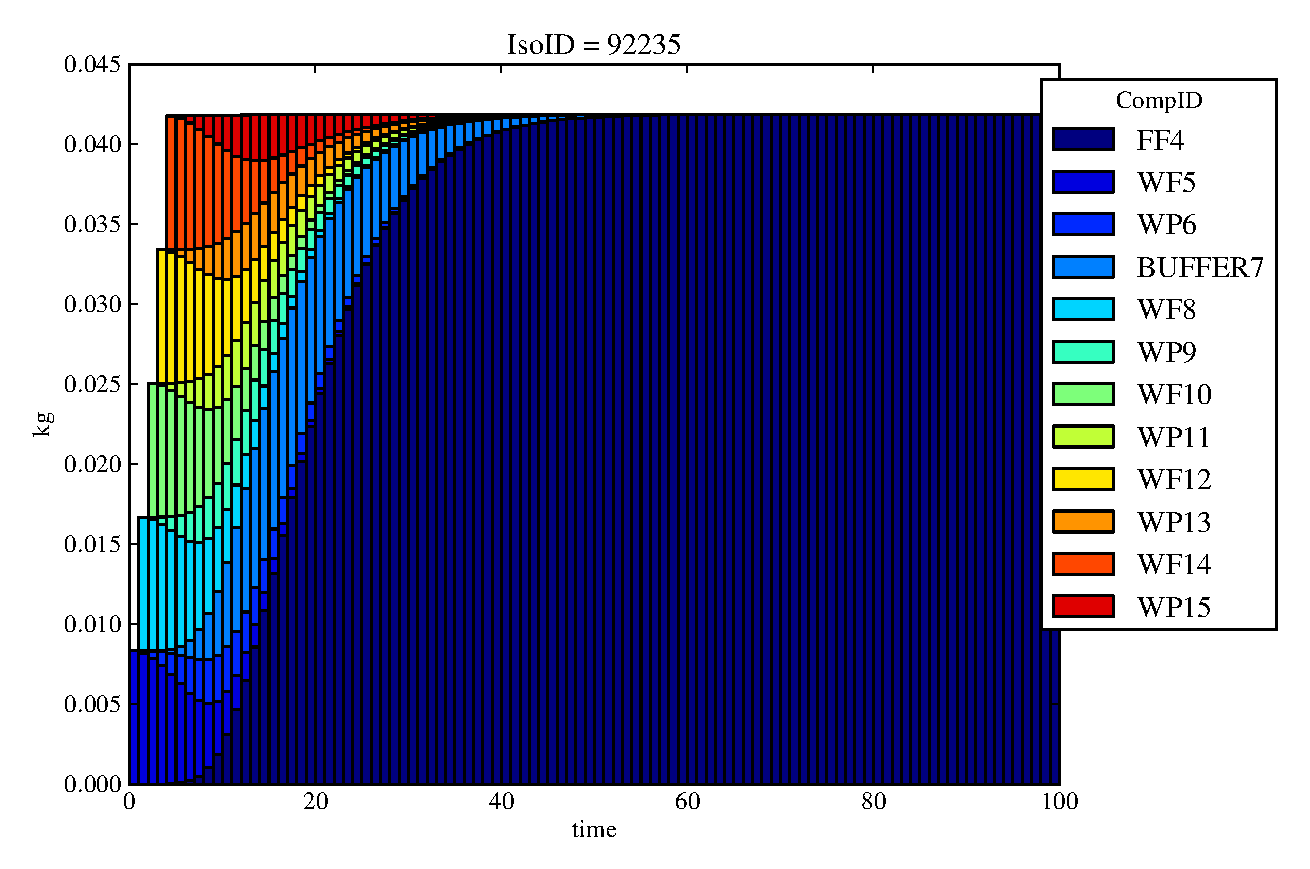
\includegraphics[width=0.6\textwidth]{./results/images/mcIII.eps}
\caption[$^{235}U$ residence. Mixed Cell Coupled Sorption and Solubility Limitation.]{
For the MCIII case in which containment is affected by solubility limitation,
        ($F_{d}=0.1$ for all components except far field), $^{235}U$ travels through waste 
        packages (WPN), their corresponding waste forms (WFN), and the surrounding 
        buffer (BUFFER7) more slowly than in the MCI case
        before permanent residence in the far field component (FF).
}
\label{fig:mcIIIall}
\end{figure}

\begin{figure}[ht]
\centering
  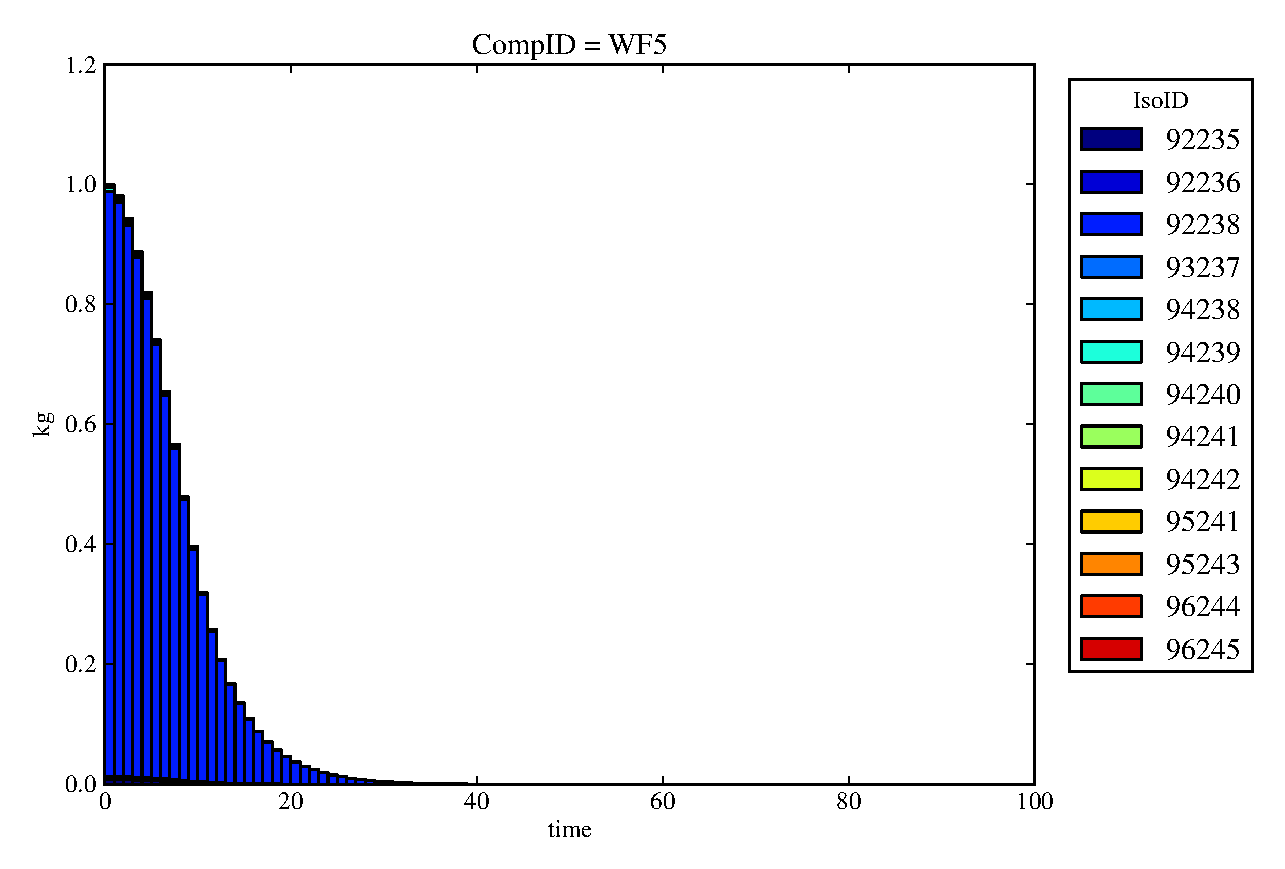
\includegraphics[width=0.6\textwidth]{./results/images/mcIII1.eps}
  \caption[Case MCIII Waste Form Contaminants.]{
          Waste Form 5 (degradation rate $F_d = 0.1[y^{-1}]$, reference solubility limit $S_{ref} = 0.001kg/m^3$) releases material with degradation.
    }
  \label{fig:mcIIIwf5}
\end{figure}


\begin{figure}[ht]
\centering
  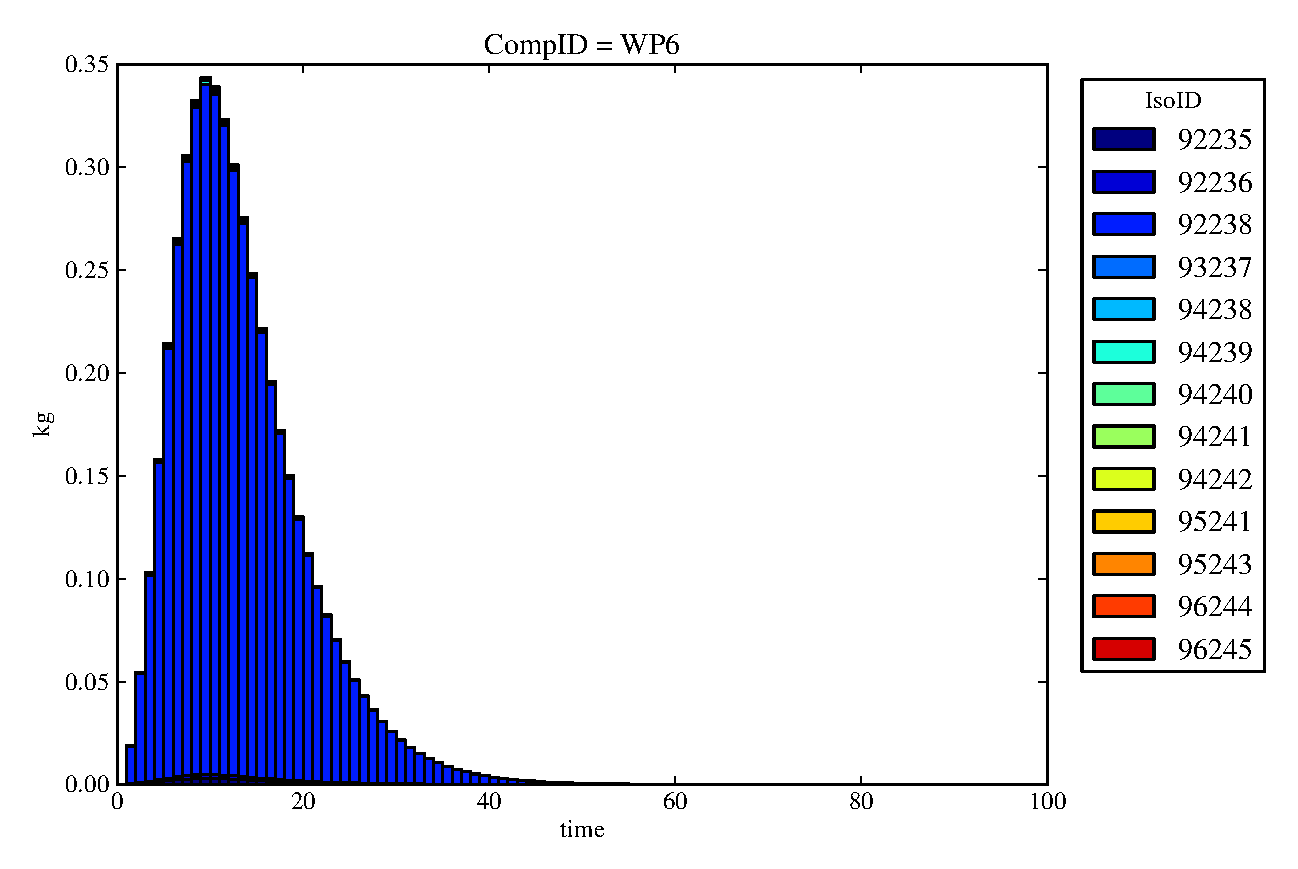
\includegraphics[width=0.6\textwidth]{./results/images/mcIII2.eps}
  \caption[Case MCIII Waste Package Contaminants.]{
          Waste Package 6 (degradation rate $F_d = 0.1[y^{-1}]$, reference solubility limit $S_{ref}=0.001kg/m^3$) receives then releases material.
    }
  \label{fig:mcIIIwp6}
\end{figure}

\begin{figure}[ht]
\centering
  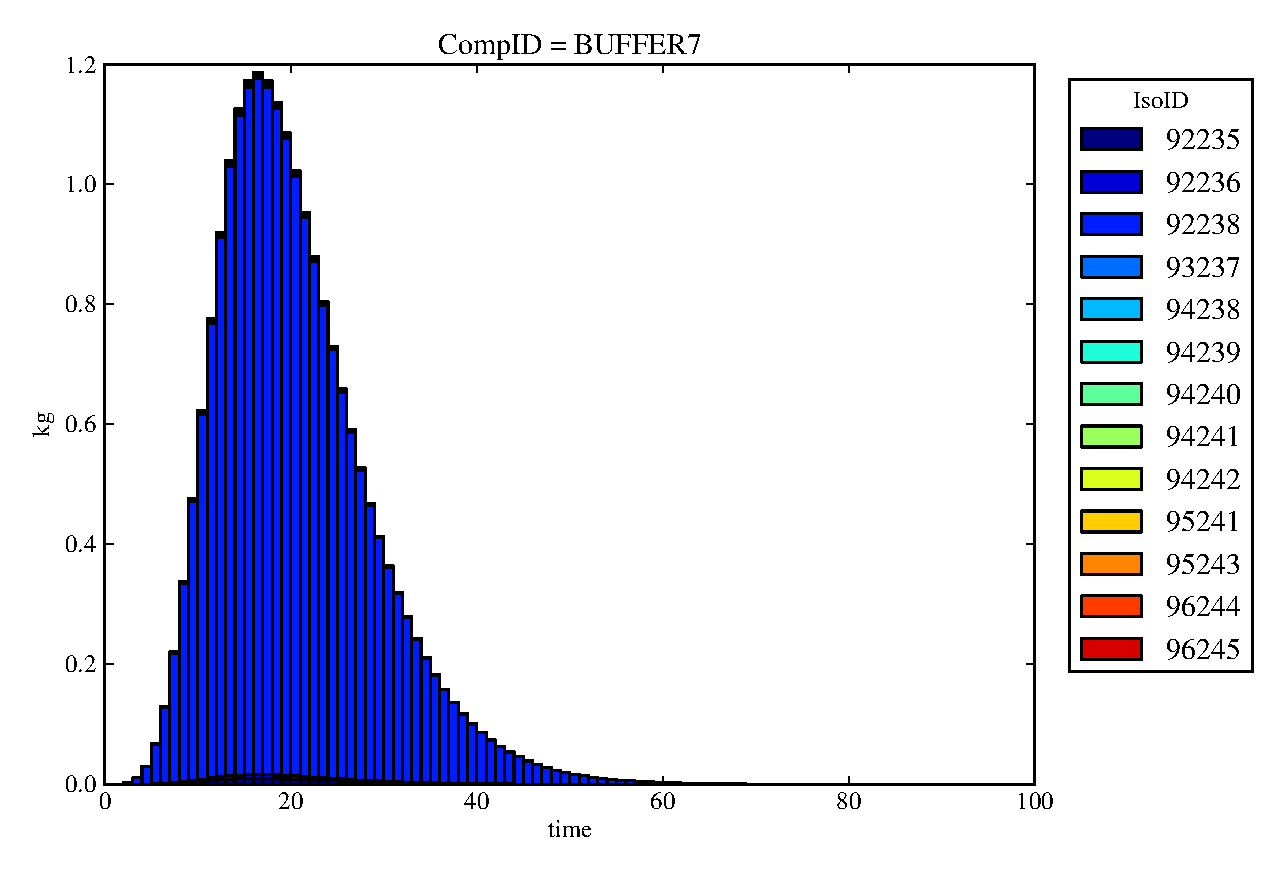
\includegraphics[width=0.6\textwidth]{./results/images/mcIII3.eps}
  \caption[Case MCIII Buffer Contaminants]{
          The Buffer, component 7 (degradation rate $F_d=0.1[y^{-1}]$, reference solubility 
        limit $S_{ref}=0.001kg/m^3$), receives and then releases material.
    }
  \label{fig:mcIIIbuff}
\end{figure}

\begin{figure}[ht]
\centering
  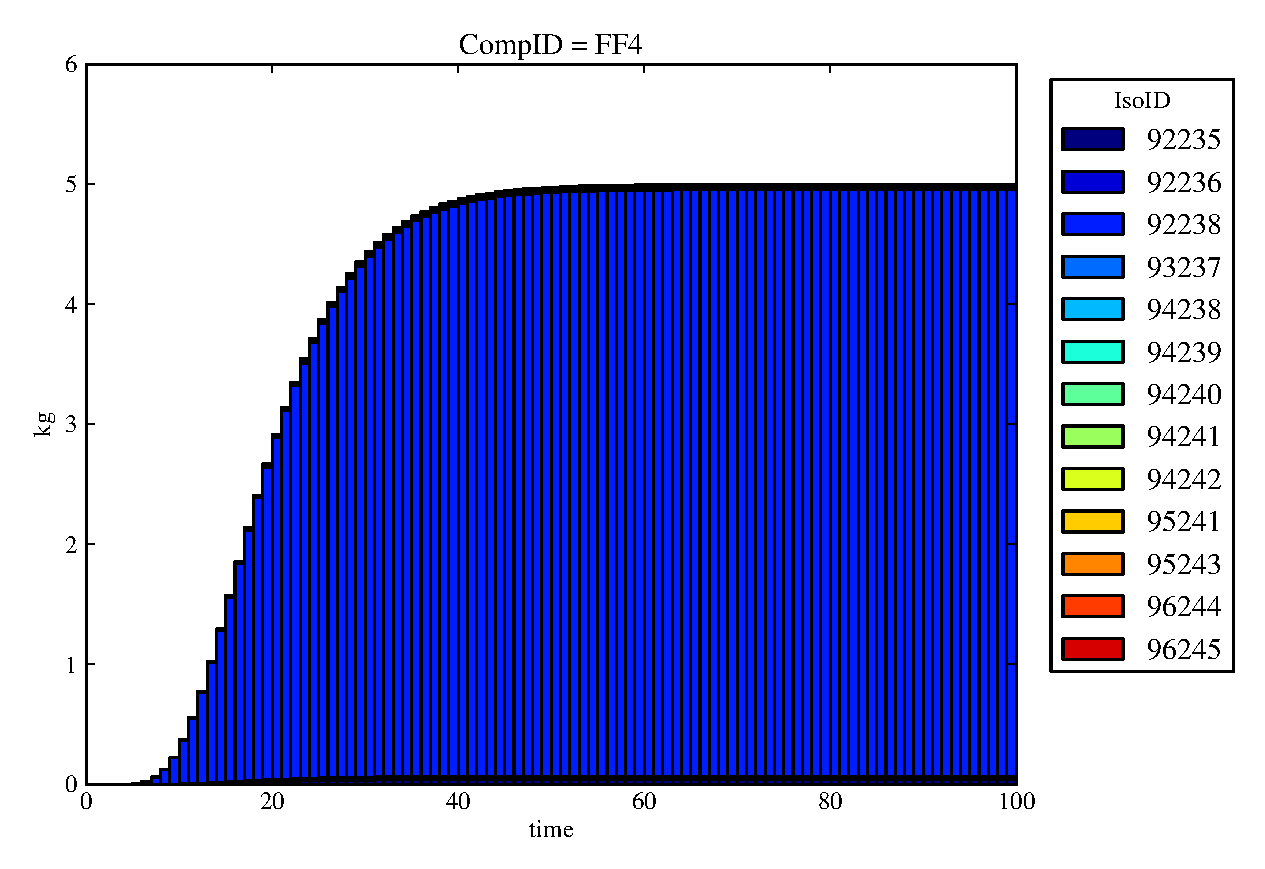
\includegraphics[width=0.6\textwidth]{./results/images/mcIII0.eps}
  \caption[Case MCIII Far Field Contaminants.]{All material is released into
        the Far Field, component 4 (degradation rate $F_d=0.0[y^{-1}]$, reference solubility limit $S_{ref} = 0.001kg/m^3$).}
  \label{fig:mcIII}
\end{figure}



\FloatBarrier



\subsection{Single Effect Parametric Analyses}
% Many parametric analysis were conducted to validate system responses 

The above multi-component simulation was conducted accross a range of 
reference solubility limits. This parametric analysis was conducted to show that, for an 
arbitrary isotope, the expected solubility limitation
behavior is captured. In the case of real isotopes in a full simulation, the 
same model will be invoked with real parameters for each isotope. Thus, the 
this model agreement is representative in all cases.

The results acheived with \Cyder were compared to the results of a parametric sensitivity 
analysis reported in \cite{huff_key_2012}. That analysis, conduced with a more 
detailed generic radionuclide transport model, showed that for solubility 
limits below a certain threshold, the dose releases were directly proportional 
to the solubility limit, indicating that the radionuclide concentration 
saturated the groundwater up to the solubility limit near the waste form.  For 
solubility limits above the threshold, however, further increase to the limit 
had no effect on the peak dose. This demonstrates the situation in which the 
solubility limit is so high that even complete dissolution of the waste 
inventory into the pore water is insufficient to reach the solubility limit.

The results in Figure \ref{fig:SolSumFactor}, from the detailed parametric 
analysis in \cite{huff_key_2012}, it is clear that for 
solubility constants lower than the saturation threshold, the transport regime is solubility 
limited and the relationship between peak annual dose and solubility limit is 
strong.  Above the threshold, the transport regime is inventory limited 
instead.

In the corresponding parametric analysis of \Cyder performance, it was shown that the 
solubility sensitivity behavior closely matched that of the \gls{GDSM} 
sensitivity behaviors. Specifically, in Figure \ref{fig:sol_result}, a sharp turnover 
is seen where the solubility limit exceeds the point at which it limits 
movement. For increased solubility limits, release remains constant.

\begin{figure}[ht]
\begin{center}
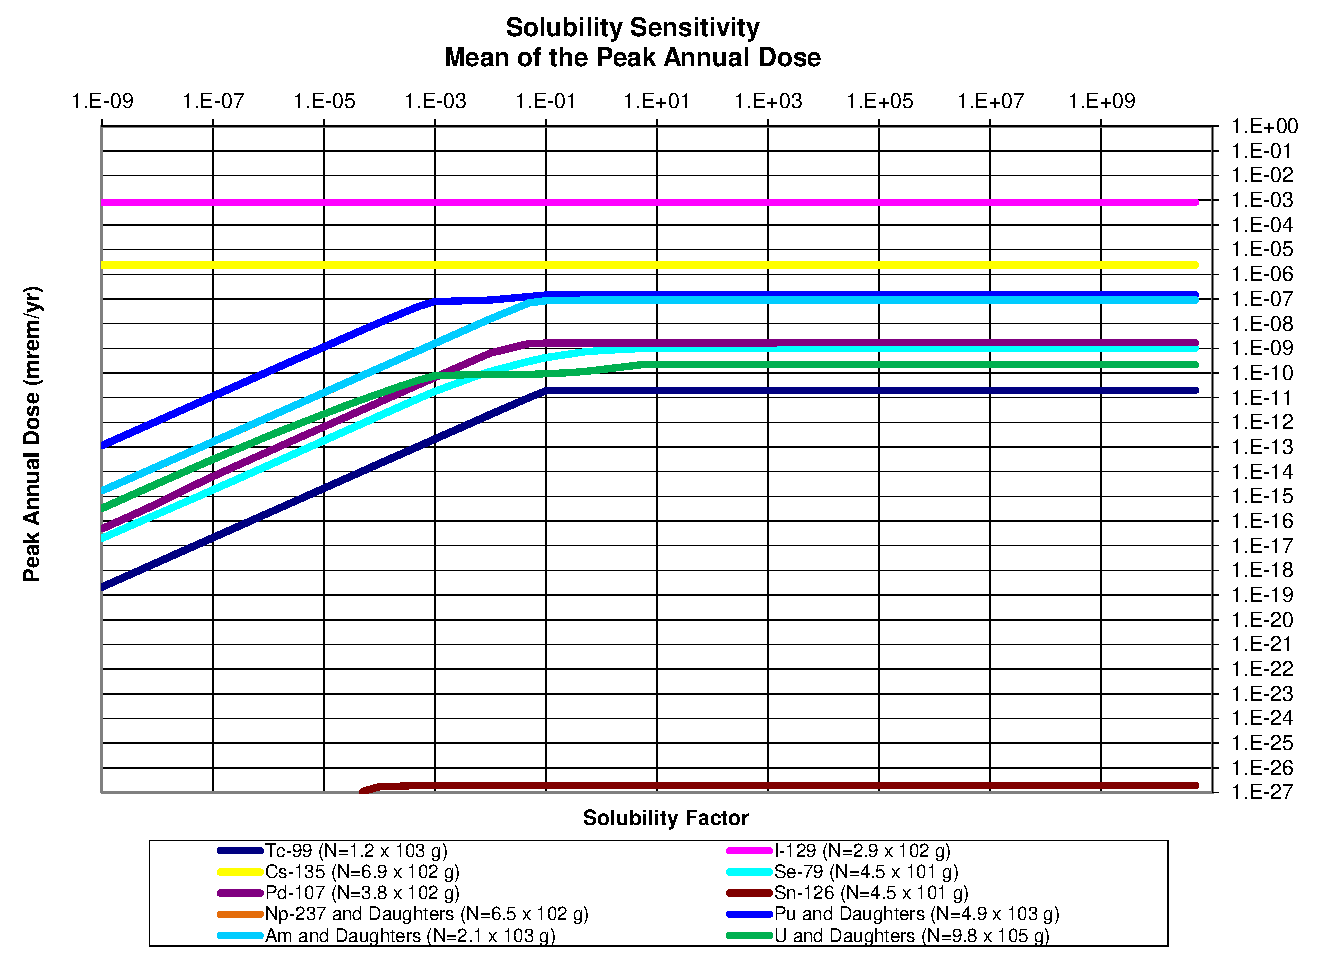
\includegraphics[width=0.7\linewidth]{./Solubility_Summary_SolFactor.eps}
\caption[Solubility factor sensitivity in GDSM Clay model]{Solubility factor sensitivity. The peak annual dose due to an inventory, $N$, of each isotope. This result was acheived with a parametric analysis using a detailed model of a generic clay repository \ref{huff_key_2012}}
\label{fig:SolSumFactor}
\end{center}
\end{figure}

%\begin{figure}[ht]
%\begin{center}
%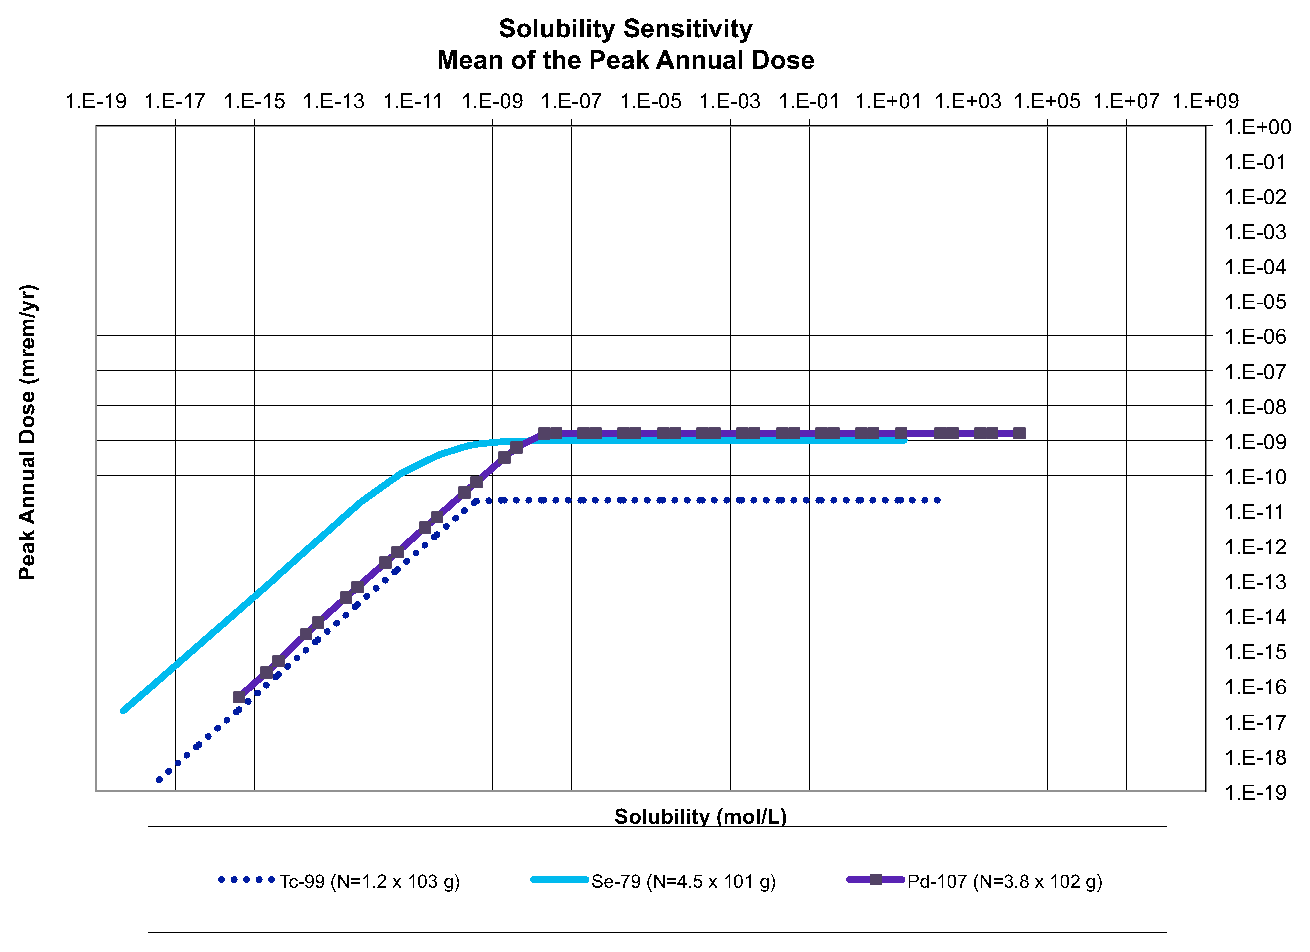
\includegraphics[width=0.7\linewidth]{./Solubility_Summary_Sol.eps}
%\caption[Solubility limit sensitivity in GDSM Clay model]{Solubility limit sensitivity. The peak annual dose due to an inventory, 
%$N$, of each isotope.}
%\label{fig:SolSum}
%\end{center}
%\end{figure}

\begin{figure}[htbp!]
\begin{center}
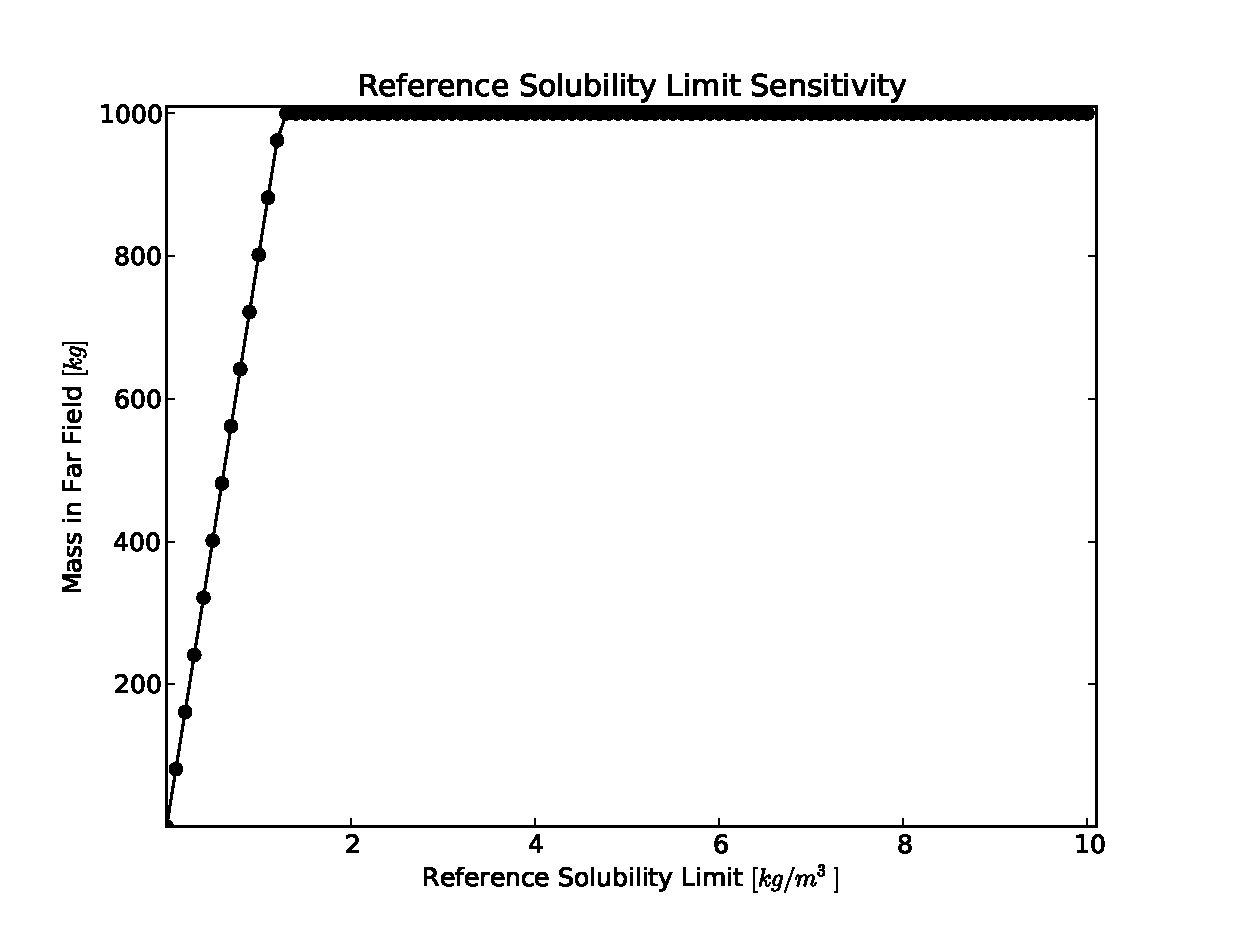
\includegraphics[width=0.7\linewidth]{./sol.eps}
\caption[Solubility Sensitivity in the Mixed Cell Model]{Sensitivity demonstration of solubility limitation in \Cyder for an arbitrary isotope assigned a variable solubility limit.}
\label{fig:sol_result}
\end{center}
\end{figure}


\FloatBarrier
\subsection{Significance}
% The existence of this code enables dynamic analysis of repository performance 
% during fuel cycle simulation.

This work has provided a flexible code for rapid mediuim fidelity calculation
of generic repository performance in the context of fuel cycle analysis.
Capable of hydrologic contaminant transport discussed here, thermal transport
demonstrated elsewhere, and integration within a fuel cycle simulation code,
\Cyder is the first of its kind.

In this work, key conceptual components and modeling methods for geologic
radioactive waste disposal were identified as part of a literature review,
dominant physics of thermal and radionuclide transport were identified by
conducting sensitivity analyses with detailed codes. Accordingly, a basic set
of abstracted models were developed and implemented within the \Cyder code.

A set of basic capabilities within the \Cyder library have been developed and
validated and an assortment of advanced features, data, testing, and plotting
capabilities are functional. The \Cyder source code in which these models are
implemented is made freely available to interested researchers and potential
model developers \cite{huff_cyder_2013}. In addition to the source code and
supporting publications, the \Cyder code is well commented and produces
clickable, browsable automated documentation with each build. That
documentation is also available online \cite{huff_cyder_2013}.

The application programming interface to this software library is intentionally
general, facilitating the incorporation of the models presented here within
external software tools in need of a multicomponent disposal system simulator.  

Furthermore, this work contributes to an expanding ecosystem of computational
models available for use with the Cyclus fuel cycle simulator. This hydrologic
nuclide transport library, by virtue of its capability to modularly integrate
with the Cyclus fuel cycle simulator has laid the foundation for integrated
disposal option analysis in the context of fuel cycle options.
